% !TeX spellcheck = cs_CZ
%=====================Kapitola: Obvody v harmonickém ustáleném stavu=======================
\chapter{Obvody v harmonickém ustáleném stavu}
  V této kapitole se seznámíme se \emph{symbolicko-komplexní metodou} (\texttt{SKM}), jež má
  základní důležitost pro teorii obvodů v harmonickém ustáleném stavu. Potom prozkoumáme vlastnosti
  jednodušších obvodů v tomto stavu a metody jejich analýzy. Posléze pojednáme o elektrickém výkon
  v obvodech a o nejdůležitějších otázkách přenosu energie \cite[s.~60]{Mayer1978}.
  
  \section{Periodické veličiny a jejich charakteristické hodnoty}
    \emph{Periodickou veličinou} nazýváme takovou veličinu $v$, jejíž závislost na čase lze
    vyjádřit periodickou funkcí, pro níž existuje konstanta $T>0$ taková, že pro každé $t$ platí
    vztah
    \begin{equation}\label{TEO:eq_harm01}
      v(t+T) = v(t),    
    \end{equation}  
    Konstanta $T$ se nazývá \textbf{perioda} resp. \emph{doba kmitu}. V aplikacích se zpravidla
    používá nejmenší kladná perioda, tzv. \emph{základní perioda}; pro stručnost budeme hovořit
    pouze o periodě. Je-li dána periodická veličina na jakémkoliv intervalu $(t_0, t_0+T)$, je tím
    zřejmě definována pro všechna $t>t_0$. Průběh veličiny $v$ na jakémkoliv intervalu délky $T$ se
    nazývá \emph{cyklem}. Počet cyklů za jednotku času (za sekundu) udává \textbf{kmitočet}, nebo
    též \emph{frekvenci} periodické veličiny
    \begin{equation}\label{TEO:eq_harm02}
      f = \frac{1}{T},
    \end{equation}
    V elektrotechnice rozdělujeme periodické veličiny do dvou skupin:
    \begin{figure}[ht!] % \ref{teo:fig029}
       \centering
       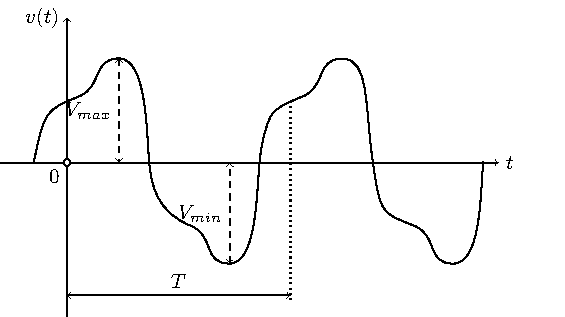
\includegraphics[width=0.8\linewidth]{teo_fig029.pdf}
       \caption{Příklad periodické veličiny $v=v(t)$ pro kterou platí $v(t+T)=v(t)$}
       \label{teo:fig029}
    \end{figure}

    \begin{figure}[ht!] % \ref{teo:fig030}
       \centering
       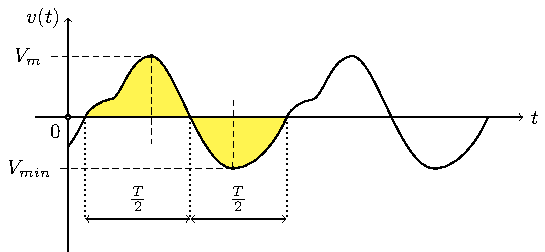
\includegraphics[width=0.8\linewidth]{teo_fig030.pdf}
       \caption{Časový průběh \textbf{střídavé veličiny} $v=v(t)$, pro kterou platí, že obsahy ploch
                v jednom cyklu nad osou $t$ a pod osou $t$ jsou totožné}
       \label{teo:fig030}
    \end{figure}

    \begin{itemize}
      \item Veličiny $v$, jež během svého cyklu \emph{změní znaménko} (obr.\ref{teo:fig029})
            nazýváme \textbf{kmitavé}. \emph{Speciálním případem} kmitavých veličin jsou
            \textbf{střídavé veličiny}, jež mají tu vlastnost, že po dobu $T/2$ jsou trvale kladné,
            po dobu $T/2$ naopak záporné a obsahy ploch omezených grafem funkce $v=v(t)$ v jednom
            cyklu nad osou $t$ a pod osou $t$ jsou \emph{totožné} (obr. \ref{teo:fig030}).
      \item Veličiny $v$, jež \emph{nemění své znaménko}, tj. jsou trvale kladné nebo trvale
            záporné (obr.\ref{teo:fig031}) nazýváme \textbf{pulzující}. \emph{Speciálním případem}
            jsou \textbf{stejnosměrné veličiny}, které nemění svou hodnotu, tj. $v=konst$
            (obr.\ref{teo:fig031} (b)).
    \end{itemize} 

    \begin{figure}[ht!] % \ref{teo:fig031}
       \centering
       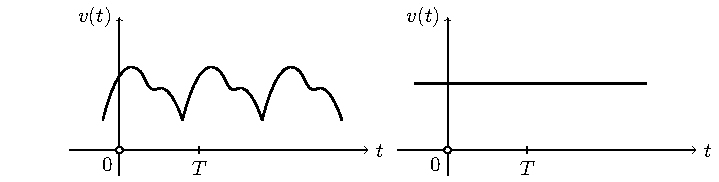
\includegraphics[width=0.8\linewidth]{teo_fig031.pdf}
       \caption{Časový průběh pulsující periodické veličiny a konstantní veličiny}
       \label{teo:fig031}
    \end{figure}

    Praktický význam mají zejména tyto hodnoty periodických veličin:
    \begin{itemize}
      \item \emph{Maximální hodnota} $V_m$ periodické veličiny $v$, tj. největší hodnota, které
            tato veličina dosahuje $v_m=\max v(t)$
      \item \emph{Minimální hodnota} $V_{min}$ periodické veličiny $v$, tj. nejmenší hodnota, které
            tato veličina dosahuje $v_m=\min v(t)$
    \end{itemize}
      
    Maximální a minimální hodnoty střídavé veličiny se nazývají též \emph{vrcholovými hodnotami}
    (kladnými nebo zápornými), obr. \ref{teo:fig029} a \ref{teo:fig030}. 
    
    \fbox{Střední hodnota} veličiny $v$ v intervalu $\langle t_i, t_j\rangle$ je 
    \begin{equation}\label{TEO:eq_harm03}
      V_s = \frac{1}{t_j-t_s}\int_{t_j}^{t_s}v(t)dt
    \end{equation}
    U periodické veličiny se spravidla počítá střední hodnota v jedno cyklu. U střídavé veličiny je
    v jednom cyklu $V_s = 0$,  a proto střední hodnotu vyjadřujeme v takovém intervalu v němž je
    $v\geq0$.
    
    \fbox{Efektivní hodnota} periodické veličiny v intervalu $\langle 0, T\rangle$ je 
    \begin{equation}\label{TEO:eq_harm04}
      V = \sqrt{\frac{1}{T}\int_{0}^{T}v^2(t)dt}
    \end{equation}   
    U periodických napětí a proudů má praktický význam především jejich efektivní hodnota.
    Efektivní hodnotu periodického proudu $i=i(t)$ procházejícího konstatním odporem $R$ lze
    interpretovat jako stejnosměrný proud $I$, při němž se za dobu $T$ vyvine v odporu $R$ stejná
    tepelná energie, jako průchodem proudu $i$. Podle \emph{Joulova-Lenzova} zákona je totiž
    \begin{equation}\label{TEO:eq_harm05}
      RI^2T = \sqrt{\frac{1}{T}\int_{0}^{T}Ri^2(t)dt}
    \end{equation}       
    z čehož lze určit $I$ v souladu s rovnicí \ref{TEO:eq_harm04}. Obdobně lze fyzikálně
    interpretovat efektivní hodnotu napětí.
    
    Střední hodnotu periodického proudu $i=i(t)$ lze fyzikálně interpretovat jako stejnosměrný
    proud $I_s$, jimž se za dobu $T$ přenese stejný náboj $Q$ jako proudem $i$:
    \begin{equation}\label{TEO:eq_harm06}
      Q = I_sT = \int_{0}^{T}i(t)dt
    \end{equation}       
    z čehož plyne $I_s$ v souladu s rovnicí \ref{TEO:eq_harm03}.  
    
    Efektivní hodnotu napětí (proudu) lze změřit např. feromagnetickým, elektrodynamickým nebo
    tepelným voltmetrem (ampérmetrem). Střední hodnotu napětí (proudu) magnetoelektrickým
    voltmetrem (ampérmetrem) a střední hodnotu výkonu elektrodynamickým wattmetrem.

    \begin{figure}[ht!] % \ref{teo:fig032}
       \centering
       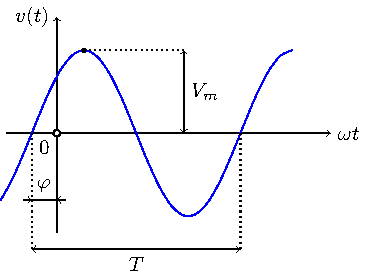
\includegraphics[width=0.8\linewidth]{teo_fig032.pdf}
       \caption{Haromincká funkce $v = V_m\cos(\omega t + \varphi)$ resp. 
                $v= V_m\cos(\omega t + \varphi')$ kde je $\varphi' = \varphi - \frac{T}{4}$}
       \label{teo:fig032}
    \end{figure}

    Střídavou veličinu $v$ lze též do jisté míry charakterizovat \emph{činitelem tvaru} $\beta$,
    \emph{činitelem výkyvu} $\gamma$ a \emph{činitelem plnění} $\alpha$ definovanými vztahy
    \begin{equation}\label{TEO:eq_harm07}
      \beta = \frac{V}{V_s}, \quad \gamma = \frac{V_m}{V}, \quad \alpha = \frac{V_s}{V_m}
    \end{equation}    
    Je zřejmé, že platí $\alpha\beta\gamma = 1$.
    
    V elektrotechnice mají velkou důležitost periodická napětí a proudy, jejichž závislost je dána
    sinusovou nebo kosinusovou funkcí, tj.
    \begin{equation}\label{TEO:eq_harm08}
      v = V_m\sin(\omega t + \varphi),
    \end{equation}        
    nebo
    \begin{equation}\label{TEO:eq_harm09}
      v = V_m\cos(\omega t + \varphi),
    \end{equation}  
    kde $V_m$, $\omega$, $\varphi$ jsou konstanty (obr. \ref{teo:fig032})
    
    Jelikož, tato napětí, resp. proudy představují \emph{harmonické kmity}, nazýváme je
    \emph{harmonicky proměnné}, nebo krátce \emph{harmonická napětí} resp. \emph{harmonická
    proudy}. Konstanta $V_m$ je maximální hodnota, či-li \emph{amplituda}, $\omega t + \varphi$ je
    \emph{fáze}, $\omega = 2\pi f = \frac{2\pi}{T}$ je \emph{úhlový kmitočet} a $\varphi$ je
    \emph{počáteční fáze} harmonické funkce.
    
    Rozdíl fází dvou harmonických veličin (stejného kmitočtu) nazýváme \emph{fázový posun}.
    
    % --------example: Efektivní hodnota výpočet -----------
    % \label{TEO:exam007}
    % !TeX spellcheck = cs_CZ
\begin{example}\label{TEO:exam007}
  Pro harmonickou veličinu, určete efektivní hodnotu, střední hodnotu, činitele tvaru, činitele
  výkyvu a činitele plnění \newline
  \textbf{Řešení:} Efektivní hodnota je:
  \begin{align}
    V &= \sqrt{\frac{1}{T}\int_0^TV_m^2\cos^2{(\omega t + \varphi)}\,dt}    \nonumber  \\
      &= \sqrt{\frac{1}{T}\int_0^TV_m^2\sin^2{(\omega t + \varphi)}\,dt} = 
         \frac{1}{\sqrt{2}}V_m \doteq 0.707 V_m   
  \end{align}
  Podrobný výpočet tohoto integrálu pomocí substituce $\omega t + \varphi=\dfrac{\alpha}{2}$ je
  poněkud zdlouhavější:
  \begin{align*}
      \omega t + \varphi=\dfrac{\alpha}{2}   
    & \rightarrow  2(\omega t + \varphi) = \alpha      \\ 
      \omega dt = \frac{1}{2}d\alpha         
    & \rightarrow dt = \frac{1}{2\omega}d\alpha
  \end{align*}
  Nesmíme zapomenout přepočítat meze $\alpha_d\lvert_{t=0}=2\varphi$ a $\alpha_h\lvert_{t=T} = 
  4\pi+2\varphi$ nového integrálu.
  \begin{align*}
    V^2  &= \frac{V_m}{2T\omega}\int_{\alpha_d}^{\alpha_h}\cos^2\frac{\alpha}{2}\,d\alpha    \\
         &= \frac{V_m}{4\pi}\int_{\alpha_d}^{\alpha_h}\frac{1+\cos\alpha}{2}\,d\alpha  
          = \frac{V_m}{4\pi}\left(\left.\frac{\alpha}{2}\right\rvert_{\alpha_d}^{\alpha_h}
          + \left.\frac{1}{2}\sin\alpha\right\rvert_{\alpha_d}^{\alpha_h}\right)             \\
         &= \frac{V_m}{4\pi}\left(2\pi+\varphi-\varphi 
          + \frac{1}{2}\sin(4\pi+2\varphi)
          - \frac{1}{2}\sin(2\varphi)\right) = \frac{V_m}{2}.  
  \end{align*}  
  Při zjednodušování integrálu je užito známého goniometrického vzorce \(\cos^2\dfrac{\alpha}{2} = 
  \dfrac{1+\cos\alpha}{2}\) a faktu \(\sin(x+2k\pi)=\sin x\)
  
  Střední hodnota kladné půlvlny je 
  \begin{align*}
    V_s &= \frac{2}{T}\int\limits_{-S\frac{T}{4}-
           \frac{\varphi}{\omega}}^{\frac{T}{4}-
           \frac{\varphi}{\omega}}{V_m\cos(\omega t +\varphi)}\,dt                            \\
        &= \frac{2}{T}\int\limits_{-\frac{\varphi}{\omega}}^{-\frac{T}{2}-
           \frac{\varphi}{\omega}}{V_m\sin(\omega t +\varphi)}\,dt                            \\
        &= \frac{2}{\pi}V_m \doteq 0,637V_m
  \end{align*}
  činitele tvaru, výkyvu a plnění jsou 
  \begin{align*}
    \beta  &=\frac{V}{V_s}   =\frac{\pi}{2\sqrt{2}}=1,111, \\ 
    \gamma &=\frac{V_m}{V}   =\sqrt{2}\doteq1.414,         \\
    \alpha &=\frac{V_s}{V_m} =\frac{2}{\pi}\doteq0,637 
  \end{align*}
\end{example}  
    %-------------------------------------------------------
      
 %--------------------------------------------------------------------------------------------------
  \section{Obvody s nastavitelnými parametry}
    V praxi se setkáváme s obvody, u nichž lze (spojitě nebo stupňovitě) nastavit odpor odporníku, 
    kapacitu kondenzátoru, vlastní nebo vzájemnou indukčnost cívek, amplitudu, fázi nebo kmitočet
    zdroje (napětí nebo proud). Nazveme je \emph{obvody s nastavitelnými parametry}.
 %--------------------------------------------------------------------------------------------------

%} % tikzset
%---------------------------------------------------------------------------------------------------